\chapter{肺门增大与纵隔阴影增宽}

肺门增大与纵隔阴影增宽是X线检查所发现的病征。在临床上,常为提示疾病诊断的线索。

肺门是由肺动脉、肺静脉、支气管淋巴结、神经及结缔组织等所组成。正常时由于心脏和大血管偏左,左侧肺门部分为左心缘遮盖,故右侧肺门较左侧肺门易于观察到。

纵隔是两侧胸腔之间、胸骨之后和胸椎之前的间隔,其中有许多重要脏器。解剖上以胸骨角平面为界,将纵隔分为上下两部分。上纵隔以气管前壁为界,分为前后两部;下纵隔在胸骨与心包之间为前纵隔,胸椎与心包之间为后纵隔,其中间部分为中纵隔。在上纵隔中有气管、食管、胸腺、大血管、胸导管、迷走神经、左喉返神经、膈神经和交感神经干。下纵隔的前部有蜂窝组织和淋巴结;其中部有心脏、心包、升主动脉、肺血管、上腔静脉的下端、主支气管和膈神经;其后部有降主动脉、奇静脉、胸导管、食管和淋巴结(图\ref{fig7-1})。因此,从纵隔淋巴结的位置,可以预测到肺感染或肿瘤原发灶的所在处。

\begin{figure}[!htbp]
 \centering
 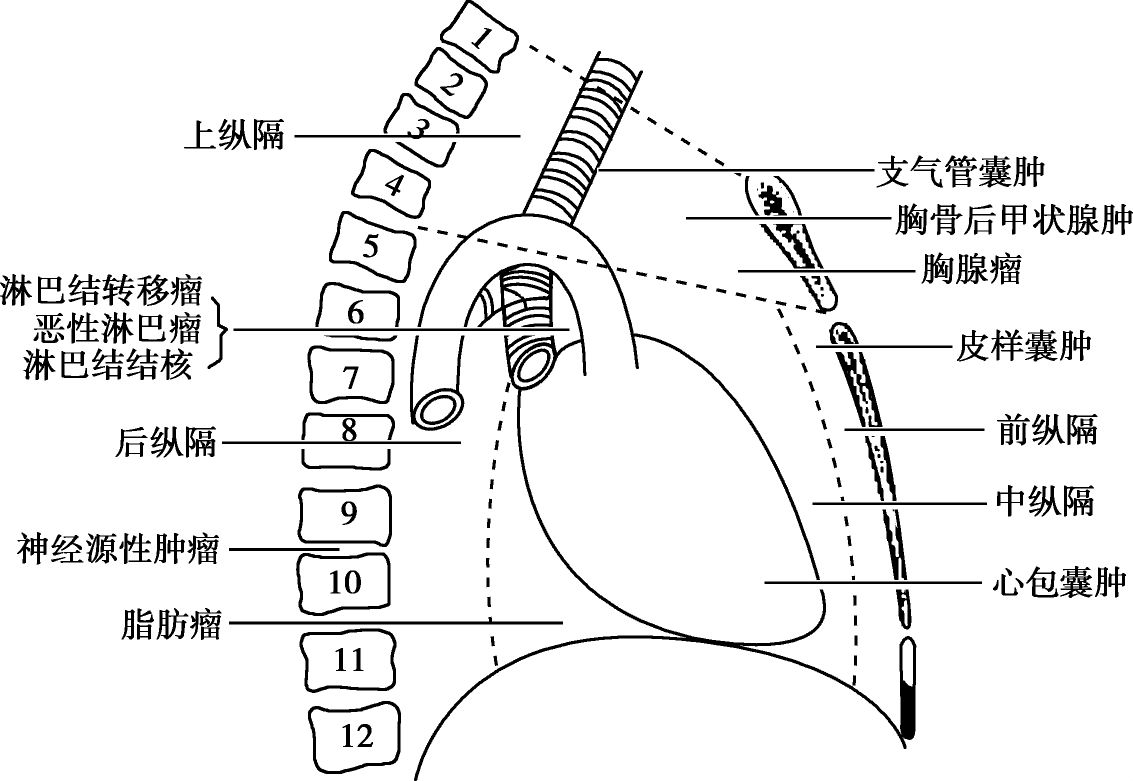
\includegraphics[width=3.9375in,height=2.6875in]{./images/Image00051.jpg}
 \captionsetup{justification=centering}
 \caption{胸部的矢状切面示意图:示纵隔与肿块的好发部位}
 \label{fig7-1}
  \end{figure} 

肺门或纵隔内任何器官和组织发生病变,均可导致肺门增大或纵隔阴影增宽。疾病分类见表\ref{tab7-1}。

\begin{table}[htbp]
\centering
\caption{肺门增大与纵隔阴影增宽疾病的分类}
\label{tab7-1}
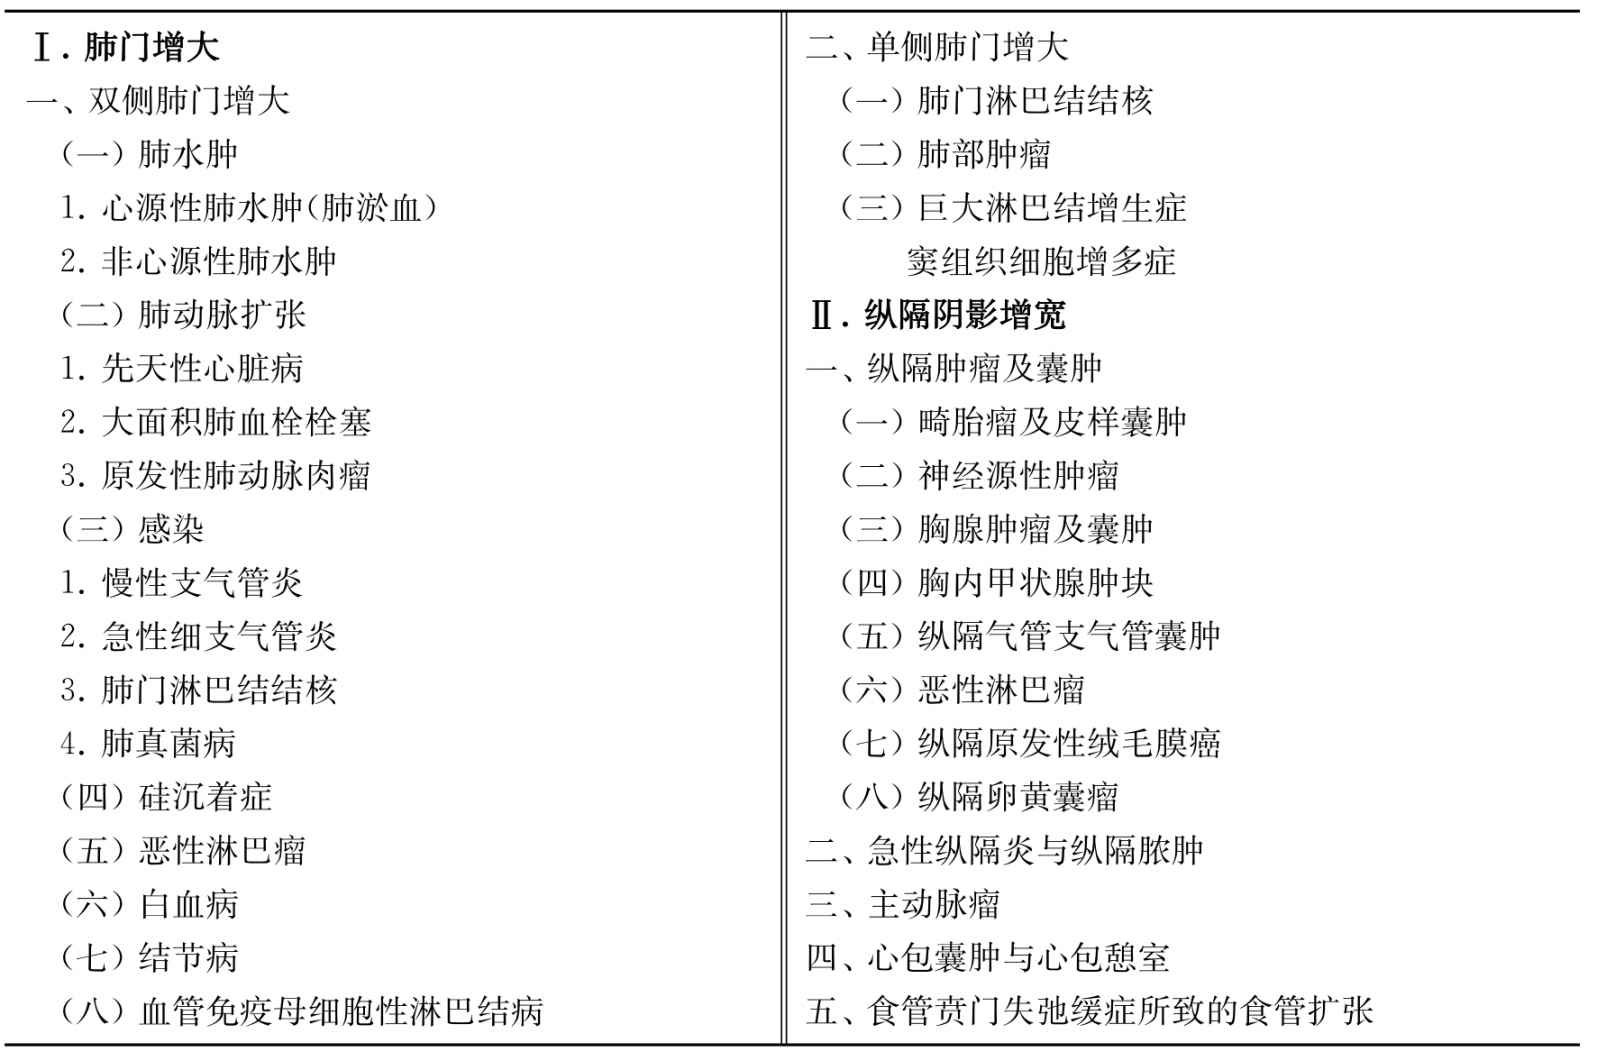
\includegraphics[width=5.89583in,height=3.91667in]{./images/Image00052.jpg}
\end{table}

\protect\hypertarget{text00080.html}{}{}

\section{26 肺门增大}

凡构成肺门阴影的任何器官、组织有病变时,均可使肺门阴影增大,但能够构成肺门增大者通常以肺门淋巴结肿大较常见。引起肺门淋巴结肿大的原因颇多,主要有原发性或转移性肿瘤、结核病、结节病、病毒性或细菌性炎症和尘肺等。

肺门增大的临床症状在小儿常较明显,而在成人则较不显著,叩诊常未能证明浊音界有异常的扩大,听诊也甚少发现支气管呼吸音。在胸椎棘突上听诊的支气管语音,正常时仅达2~3胸椎,而在肺门增大时可达5~6胸椎(D'Espine征),但这项体征在成人远不及小儿明显。发作性、痉挛性类似百日咳的咳嗽,常提示肺门增大的存在。

肺门增大的诊断需依靠X线检查,而鉴别诊断则必须联系临床情况。在X线检查时鉴别肺门属正常抑或病理性增大,有时颇为困难。如仅根据测量肺门阴影的大小,不能发现早期病变,只能观察到肺门血管和支气管的结构形态,从其密度和形态的改变来判断。CT与MRI对观察肺门大支气管、血管和肿大的淋巴结有重要诊断价值。构成肺门阴影增大的原因很多,各种病变表现不同,有些疾病既可引起一侧肺门增大,也可引起两侧肺门增大。

在鉴别诊断上区分为单侧性与双侧性仍有一定的意义。

\subsection{26.1 双侧肺门增大}

\subsubsection{一、肺水肿}

\paragraph{(一)心源性肺水肿}

主要见于由风湿性心瓣膜病、高血压性心脏病、冠状动脉硬化性心脏病、心瓣膜功能障碍、急性重症心肌炎等引起的充血性心力衰竭,导致薄壁的肺静脉扩张引起肺淤血。X线征象是双侧肺门阴影增大和肺纹理粗乱,肺野透亮度普遍降低。如并发肺泡内渗出液,则肺门周围肺野密度增高,但肺门搏动不明显。透视下可见心脏增大。听诊双肺底中、小湿啰音与心瓣膜病理性杂音。B型利钠肽(BNP)>400ng/L,N末端B型利钠肽原(NT-proBNP)>1500ng/L,则心衰可能性很大,其阳性预测值为90\%。若BNP/NT-proBNP水平正常或偏低,则基本可排除急性心衰的可能性。此外,血流动力学监测心源性肺水肿时肺毛细血管楔压(PCWP)>18mmHg,心输出量CO<5L/min,心排指数(CI)<3.0~5.0L/(min·m\textsuperscript{2}
),脉搏指示剂连续心排血量监测(PICCO)显示:血管外肺水指数(ELWI)3.0~7.0ml/kg,在正常范围。

\paragraph{(二)非心源性肺水肿}

非心源性肺水肿的病因有:①肺毛细血管流体静水压增高,除各种原因引起的左心衰竭外,主要见于输液过量、肺静脉闭塞性疾病;②肺毛细血管通透性增加,主要见于病毒性肺炎、急性呼吸窘迫综合征(ARDS)、尿毒症、吸入性肺炎、血循环毒素(蛇毒等),吸入有害气体(光气、臭气、氮氧化合物)、过敏性肺泡炎;③血浆胶体渗透压减低,见于肝肾疾病、蛋白丢失性肠病、营养不良性低蛋白血症;④淋巴回流障碍。X线表现为以肺门为中心的蝶状或片状模糊阴影。肺功能检查提示肺顺应性下降,小气道闭合气量值增高。大部分非心源性因素所引起的肺水肿,其PCWP<18mmHg,心输出量CO>5L/min,心排指数CI>3.0L/(min·m\textsuperscript{2}
)。PICCO显示:血管外肺水指数(ELWI)>10ml/kg。

\subsubsection{二、肺动脉扩张}

\paragraph{(一)左向右分流的先天性心脏病}

肺动脉扩张是由肺循环血量增加所引起,最常见于有体循环血液分流至肺循环的先天性心脏病(如房间隔缺损、室间隔缺损、动脉导管未闭、鲁登伯综合征、艾森曼格综合征),肺静脉畸形引流、特发性肺动脉扩张等情况。

X线胸片上显示肺门的肺动脉及其分支明显增大,轮廓清楚。透视下可见扩张的肺动脉搏动明显。如在房间隔缺损、动脉导管未闭等病例中,往往出现肺门血管收缩期膨胀性搏动,形成所谓肺门舞蹈(肺门搏动),是诊断肺动脉扩张的重要体征。根据上述的X线检查所见,可与肺门淤血及肺门部淋巴瘤相区别。但直接位于主动脉上的淋巴瘤,可能伴有搏动(传导性搏动)而引起混淆,须注意观察区别。

\paragraph{(二)急性大面积肺血栓栓塞}

急性大面积肺血栓栓塞(massive
PTE)指:①收缩压<90mmHg或较平时下降≥40mmHg,持续时间≥15分钟,排除其他致血压下降原因;②影像学显示栓塞部位≥2个肺叶或7个肺段,符合上述2项任意1项者,即为大面积PTE,也即高危PTE;急性中危PTE(次大面积PTE):非达到大面积PTE标准,但有右心功能不全表现;急性低危PTE(小面积PTE):未达到大面积和次大面积标准PTE者。

急性大面积PTE的X线胸片也可表现为双肺门阴影增大,肺动脉段突出或瘤样扩张,右心(房室)扩大征,右下肺动脉干增宽或伴截断征;区域性肺纹理纤细、稀疏,肺透亮度增加,未受累部分可呈现纹理相应增多。如发生肺梗死,表现为局部肺野呈楔形浸润阴影,尖端指向肺门。但仅凭X线胸片不能确诊或排除本病,应结合病史(如下肢深静脉血栓形成)及危险因素、症状(如一过性血压下降,呼吸困难、胸痛、咯血等)和其他检查加以鉴别。

肺栓塞在CT上直接征象为肺动脉内低密度充盈缺损,部分或完全包围在不透光的血流之间(轨道征),或骑跨在左右肺动脉内的血栓(马鞍征),见图\ref{fig7-2},图\ref{fig7-3},或呈完全充盈缺损,远端血管不显影;间接征象包括肺野楔形条带状高密度区或盘状肺不张,中心肺动脉扩张及远端血管分支减少或消失等。CT肺动脉造影应结合患者临床可能性评分进行判断。低危者如果CT结果正常,即可排除PTE;高危者,即使CT结果正常也不能除外单发的亚段PTE,需进一步结合下肢静脉超声、核素肺通气/灌注扫描或肺动脉造影等检查明确诊断。

\begin{figure}[!htbp]
 \centering
 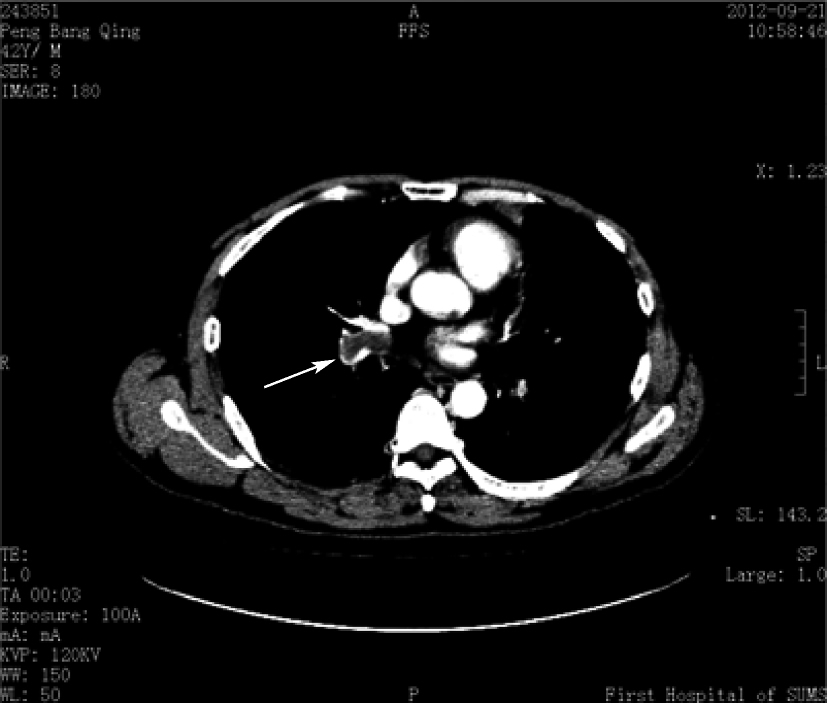
\includegraphics[width=2.75in,height=2.33333in]{./images/Image00053.jpg}
 \captionsetup{justification=centering}
 \caption{肺动脉内充盈缺损(轨道征)}
 \label{fig7-2}
  \end{figure} 

\begin{figure}[!htbp]
 \centering
 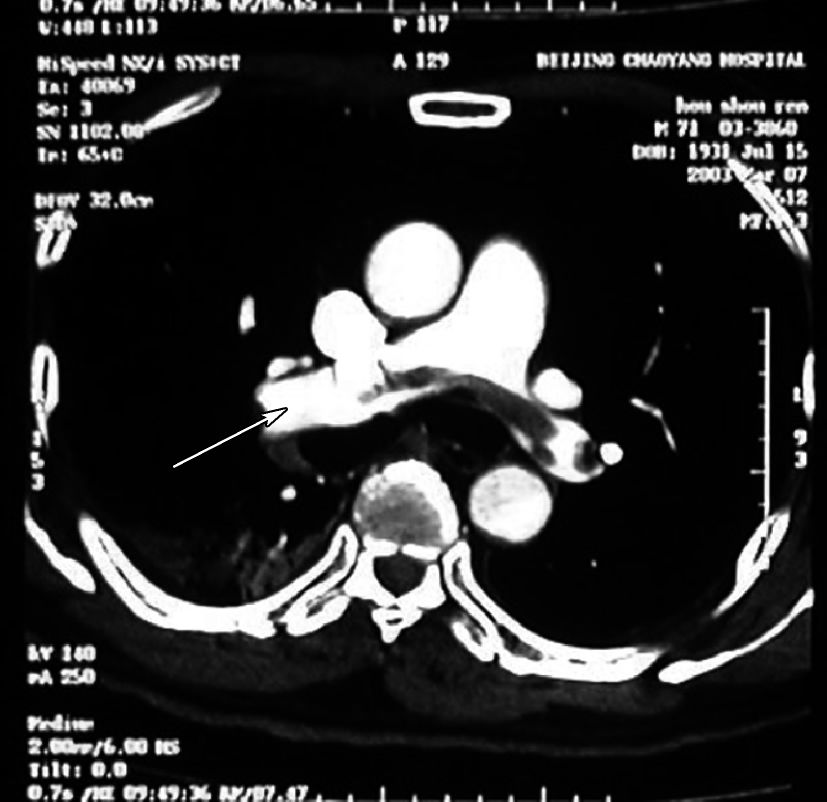
\includegraphics[width=2.41667in,height=2.34375in]{./images/Image00054.jpg}
 \captionsetup{justification=centering}
 \caption{骑跨在左右肺动脉内的血栓(马鞍征)}
 \label{fig7-3}
  \end{figure} 

\paragraph{(三)原发性肺动脉肉瘤}

原发性肺动脉肉瘤(primary arterial
sarcoma,PAS)是一种罕见的恶性肿瘤,在临床上极易与肺栓塞等肺血管疾病相混,前者抗凝治疗无效或加重。PAS的男女发病率大致相等,发病年龄在13~86岁,多为中年患者,确诊依赖手术病理学检查。胸部放射影像学表现多为:①肺门影扩大(占53\%),为扩张的肺动脉或肿物对肺组织的侵占,常被误诊为肺门淋巴结肿大;②肺内结节影(40\%),为肿瘤的直接侵犯及(或)转移所致;③心脏及(或)心包影扩大(33\%);④肺动脉远端血管影稀疏(18\%),肺动脉造影示肺动脉干及其分支充盈缺损,平均右室收缩压高达74mmHg,平均肺动脉压超过25mmHg,核素的通气及(或)灌注检查均示灌注异常;⑤肺门动脉影进行性扩大呈动脉瘤样扩张,而没有下肢及盆腔静脉系统血栓形成。与胸部X线片相比,增强胸部CT肺动脉造影对诊断PAS临床意义较大,造影多表现为主肺动脉及左、右肺动脉甚至右心室流出道内大块充盈缺损影,管腔外浸润影。见图\ref{fig7-4}。

\subsubsection{三、感 染}

\paragraph{(一)慢性支气管炎}

慢性支气管炎常引起肺门阴影增大,且常为此病表现之一。X线检查发现肺纹理普遍增多、紊乱、增厚、模糊,尤以下肺显著,并可见支气管及支气管周围呈索状、点状或斑块状阴影,肺门阴影加重,往往伴有肺气肿。

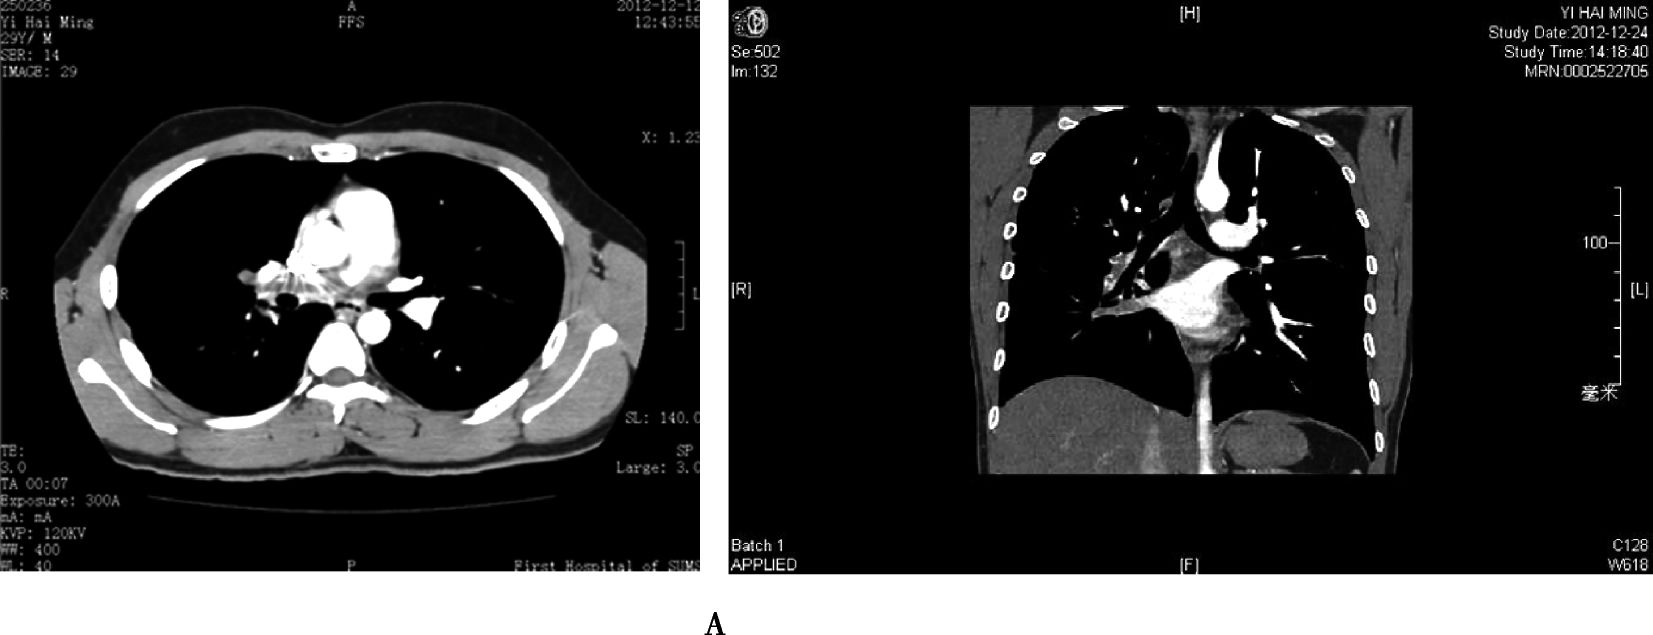
\includegraphics[width=5.54167in,height=2.15625in]{./images/Image00055.jpg}

\begin{figure}[!htbp]
 \centering
 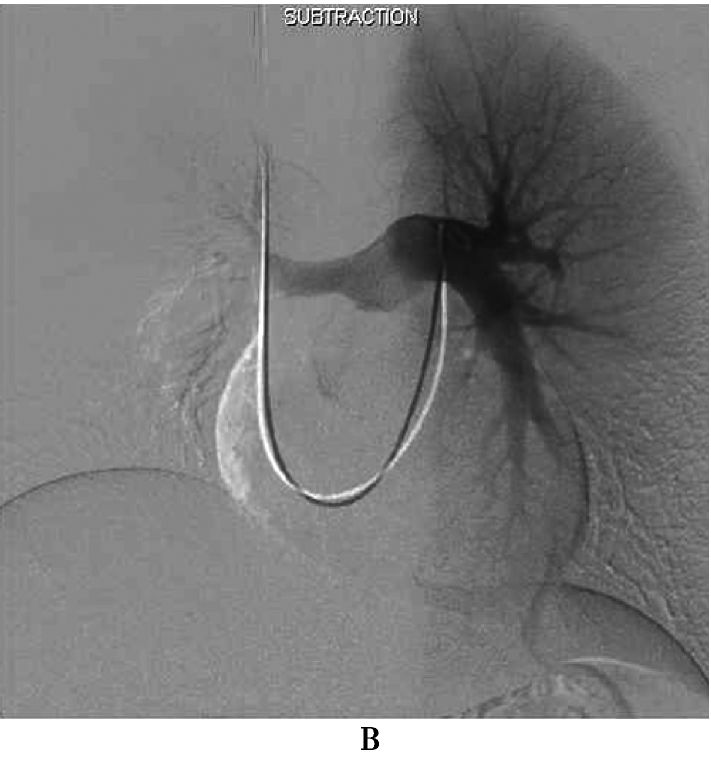
\includegraphics[width=2.36458in,height=2.55208in]{./images/Image00056.jpg}
 %\captionsetup{justification=centering}
 \caption{患者男,29岁,曾误诊为右肺动脉及分支PTE患者,先后溶栓2次,抗凝治疗无效,反复胸闷气促,后来拟行右肺动脉剥脱术,术中于中间段动脉内切取部分肿物送冰冻病理,报告为内膜肉瘤,遂行右全肺切除术。术后一般情况好\\ A.右肺动脉主干、右肺上、中、下叶动脉及其分支栓塞并动脉瘤样扩张;B.肺动脉造影+测压示右肺动脉主干充盈缺损,右肺中下叶动脉闭塞,肺动脉干压力35/17(26)mmHg,右肺动脉压37/16(26)mmHg,右室压21mmHg,右房压7mmHg,上腔静脉压7mmHg}
 \label{fig7-4}
  \end{figure} 



\paragraph{(二)急性细支气管炎}

是一种以病毒为主的感染性细支气管炎,多发生于2岁以内的婴幼儿,偶见于年长儿童和成人。临床上以呼吸窘迫、喘吼、呼气阻塞和缺氧为特征。X线检查肺透亮度增加,肋间隙增宽,横膈平坦。双侧肺门阴影增大,肺纹理增多、增粗,支气管周围有自肺门起始的密度不均匀、不规则线状阴影。

\paragraph{(三)肺门淋巴结结核}

肺门淋巴结结核是原发型肺结核的主要组成之一,一般发生于儿童或青少年。成人病例大多来自农村或少数民族地区移居城市的人。

原发型肺结核的肺内原发病灶通常吸收较快,而较多见的是遗留下来的所属肺门淋巴结结核------即支气管淋巴结结核。随着病程的进展和机体抵抗力的不同,在X线胸片上表现为结节型与浸润型两大类。结节型表现为肺门区域突出圆形或卵圆形高密影,可见钙化灶。浸润型表现为肺门阴影增宽与边缘模糊,且向肺实质扩展。在活动性肺门淋巴结结核病例中,都有不同程度的呼吸道与结核中毒症状,如咳嗽、咳痰、胸痛、不规则发热或微热、乏力、盗汗等。血沉常加快。经抗结核治疗后,病灶吸收、痊愈,最后发生纤维化与钙质沉着。

本病在鉴别诊断上须注意与中央型支气管癌、纵隔原发性肿瘤、恶性淋巴瘤、结节病等相区别。诊断主要采用排除诊断法。恶性淋巴瘤发展比较迅速,并可伴有肝、脾大,症状较重。中央型支气管癌也可引起肺门肿块,但较常引起进行性支气管腔狭窄、充盈缺损及管腔外肿块(淋巴结转移,尤其晚期病例),而致食管压迫移位及膈神经麻痹等现象。结核菌素试验在活动性结核病时常呈强阳性,在与肿瘤、恶性淋巴瘤及结节病的鉴别诊断上有一定价值。诊断性抗结核治疗疗效的意义更大。

肺门淋巴结结核是否为活动性,不能只凭一次的X线检查与临床检查结果作出定论,须依靠一系列的X线摄片和胸部CT检查。如X线征象在数周或数月之内发生改变,不论恶化或好转,也可认为有活动性或曾有活动性。比较困难的是判断已痊愈的肺门淋巴结结核,这时肺门通常呈现无明显界限的条纹状,须与慢性非特异性炎症区别。这些病例有无活动性,可依靠一系列的X线摄片和胸CT检查作对比,并参考血F常规与血沉测定。如发现肺门区域内有钙化阴影,一般可确定为已痊愈的肺门淋巴结结核。

\paragraph{(四)肺真菌病}

肺部真菌感染时,肺门阴影常有单侧性或双侧性肿大,肺部并可呈现斑片状、大片状或圆形阴影,而这些表现无特异性,易与肺部炎症、肺结核、肺肿瘤、结节病等混淆。若存在以下情况应考虑肺部真菌病的可能性:①肺门阴影增大被诊为支气管炎或肺炎,经长期抗生素治疗无效或加重;②若有长期使用糖皮质激素、免疫抑制剂、放射治疗等病史,出现肺部感染的症状或体征;③血1,3-β-D-葡聚糖抗原检测、半乳甘露聚糖检测等阳性或定量检测水平升高;④痰、尿、粪便、分泌物、血液、脑脊液等涂片、培养、组织检查,找到真菌孢子及菌丝,是诊断的重要依据。

\subsubsection{四、硅沉着病}

硅沉着病常引起双侧肺门阴影对称性增大,密度增高,以支气管旁淋巴结肿大为明显,偶尔可在其周围发生钙化,如“蛋壳”样(约5\%病例有此征象),对诊断上有一定帮助。此病最明显的改变是肺野可见多发性结节状阴影(硅沉着症结节)、肺纹理扭曲或呈网状阴影或(及)大片融合病灶,以及继发胸膜增厚、肺气肿等改变。

在硅沉着病的早期,有时仅发现支气管旁淋巴结肿大,而肺部结节不明显。矽尘职业接触史提示重要的诊断依据。

\subsubsection{五、恶性淋巴瘤}

胸部淋巴瘤包括非霍奇金淋巴瘤与霍奇金淋巴瘤,其中以前者为主。根据胸部淋巴瘤的起源不同分为三类:①胸部继发性淋巴瘤;②胸部原发性淋巴瘤;③与免疫缺陷有关的胸部淋巴瘤。继发性胸部淋巴瘤发生率较高,其中霍奇金淋巴瘤胸部病变发生率为15\%~40\%。霍奇金淋巴瘤可引起肺门及纵隔的气管、支气管旁和气管分叉部的淋巴结肿大,在X线胸片上呈结节状或分叶状阴影,边界清楚,密度均匀,一般无钙化,大多数位于前纵隔,为双侧性肿大,但不对称。肿物可压迫食管或气管、支气管,使其移位或变窄,有时肺野可出现浸润性病变,也可侵犯胸膜,出现胸腔积液。对于不对称而境界清楚的肺门淋巴结肿大,应多注意本病。如无浅表淋巴结肿大,则诊断较困难。如患者同时有周期热、外周血淋巴细胞数减少(淋巴细胞增多不支持本病)与嗜酸性粒细胞增多,须考虑此病。如患者仅有肺门淋巴结肿大,而经2~6个月之后,尚未见有颈、腋窝等处淋巴结肿大者,则霍奇金淋巴瘤的可能性小。

非霍奇金淋巴瘤引起肺部病变,以肺结节为主要表现,结节大小不一,单个或多发,一侧或两侧,有时可见空洞,多呈偏心分布;较大的肿块实变中常见到含气支气管征,此种改变多为纵隔或肺门淋巴瘤直接蔓延的结果。

浅表淋巴结活检对本病的诊断有决定性意义。本病对氮芥类药物及深部X线照射治疗相当敏感,对高度怀疑的病例可作诊断性治疗,如治疗后肺门阴影显著缩小或消失,则强力支持此类恶性淋巴瘤的诊断。

\subsubsection{六、白血病}

白血病也类似恶性淋巴瘤,可引起双侧肺门淋巴结肿大,常为对称性,常累及纵隔和支气管旁的淋巴结。有些病例可合并肺实质浸润与胸腔积液。淋巴细胞性白血病导致的肺门阴影增大较粒细胞性白血病为多见。白血病胸部浸润的X线表现形式多种多样,可几种表现形式同时存在:表现为肺间质性改变、纵隔或肺门肿大、肺内多发粟粒灶、肺内结节灶及心脏、心包、胸膜受累等,但以肺间质性改变最为常见,纵隔、肺门、腋窝淋巴结肿大的发生率次之。进行性贫血、发热与出血倾向,有助于提示此病诊断。确诊依赖于骨髓细胞学检查或浅表淋巴结活检。

\subsubsection{七、结节病}

结节病(sarcoidosis)是一种原因未明、多器官受累的肉芽肿性疾病,其特征为病变部位T细胞和单核巨噬细胞积聚、活化和非干酪性类上皮肉芽肿代替正常组织结构。罹患年龄以20~45岁为多,女性略多于男性。2/3患者无症状,是偶然X线检查时被发现。

肺脏和胸内淋巴结是结节病最常累及的部位(>90\%)。肺结节病合并肺外结节病的情况,国内统计资料:浅表淋巴结肿大37.17\%(385/1020),皮肤病变19.7\%,其中皮下结节9.3\%(74/798),皮损10.4\%(83/798)。肝脏9.0\%(46/512),眼睛19\%(57/300),腮腺3.3\%
(24/729)。肺结节病大多有淋巴结受累,周围淋巴结的受累率达71\%。周围淋巴结受累以颈前、颈后、锁骨上多见,腹股沟、腋窝、肘窝次之。病因迄今尚未明确。

胸部X线的典型表现为双肺门及纵隔淋巴结对称性肿大,可伴有肺内结节状、网状或斑片状阴影。脾脏和腹膜后淋巴结也受累(图\ref{fig7-5})。

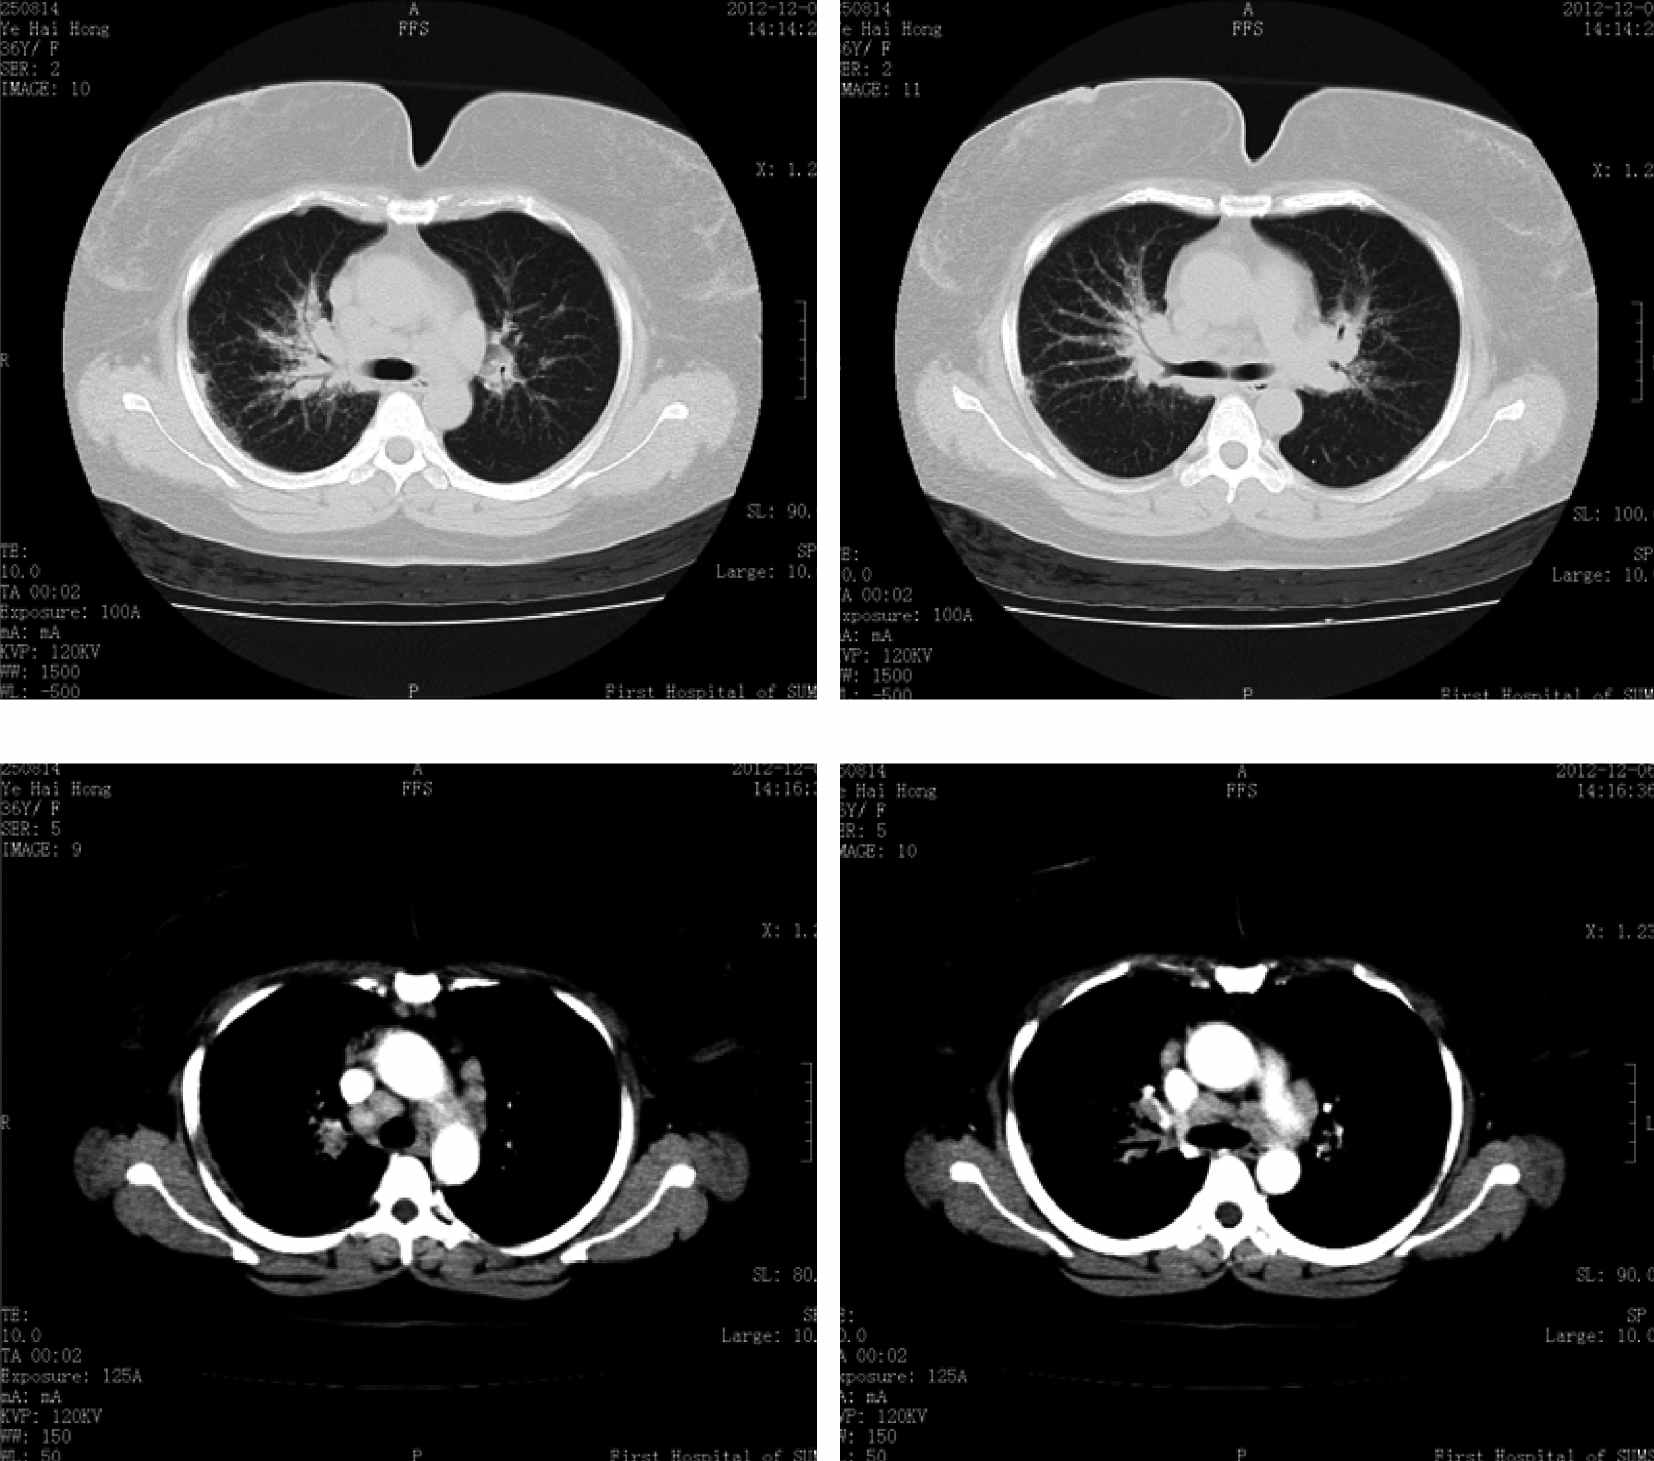
\includegraphics[width=5.51042in,height=4.86458in]{./images/Image00057.jpg}

\begin{figure}[!htbp]
 \centering
 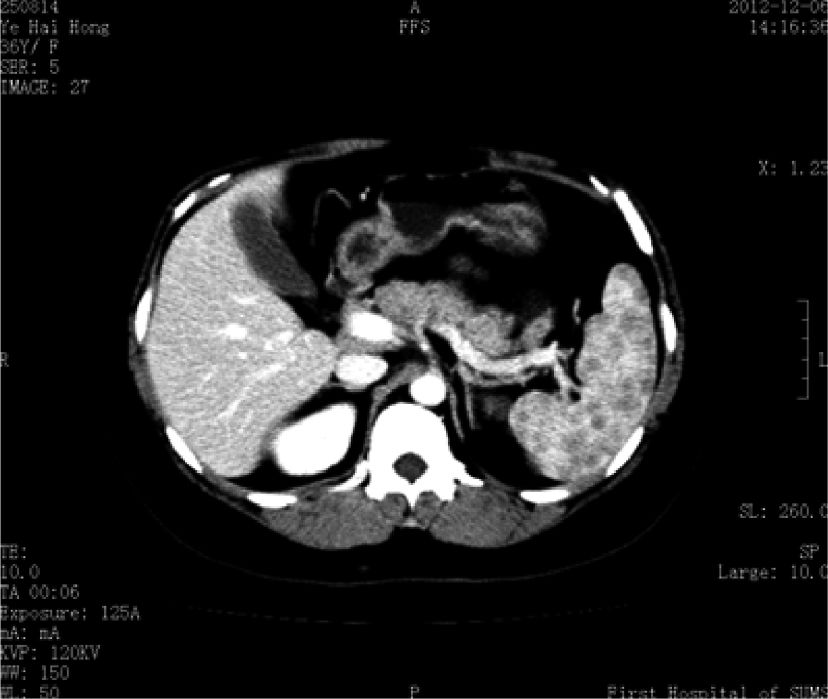
\includegraphics[width=2.75in,height=2.32292in]{./images/Image00058.jpg}
 %\captionsetup{justification=centering}
 \caption{结节病患者在肺、纵隔、脾、腹膜后影像学表现:双肺弥漫分布1~2mm大小不一斑点状影,边缘不清。双侧肺门及纵隔内见多数大小不等淋巴结影,最大者约14mm,部分融合,以右侧肺门显著,未见钙化。双肺见支气管壁增厚,由肺门向外周放射分布,周围肺实质见粟粒状小结节。脾脏多发低密度结节,腹膜后淋巴结肿大}
 \label{fig7-5}
  \end{figure} 

临床表现和自然进程差异很大。2/3患者无症状而偶然X线检查时被发现。主要表现在呼吸系统,咳嗽、气短、或胸痛。可有低热、乏力、盗汗、纳差、肌肉酸痛、皮肤病损、眼部病变等。依据表现结节病分为:①伴结节红斑的急性结节病,以急性发作的结节红斑和双肺门淋巴结肿大为表现,常伴发热、多关节炎和葡萄膜炎,即Lofgren综合征。②肺结节病,其在肺内表现见表\ref{tab7-2}\footnote{*表中可见以肺间质纤维变和网状影较多。}。③肺外结节病,约占20\%。

\begin{table}[htbp]
\centering
\caption{465例肺结节病的肺内病变}
\label{tab7-2}
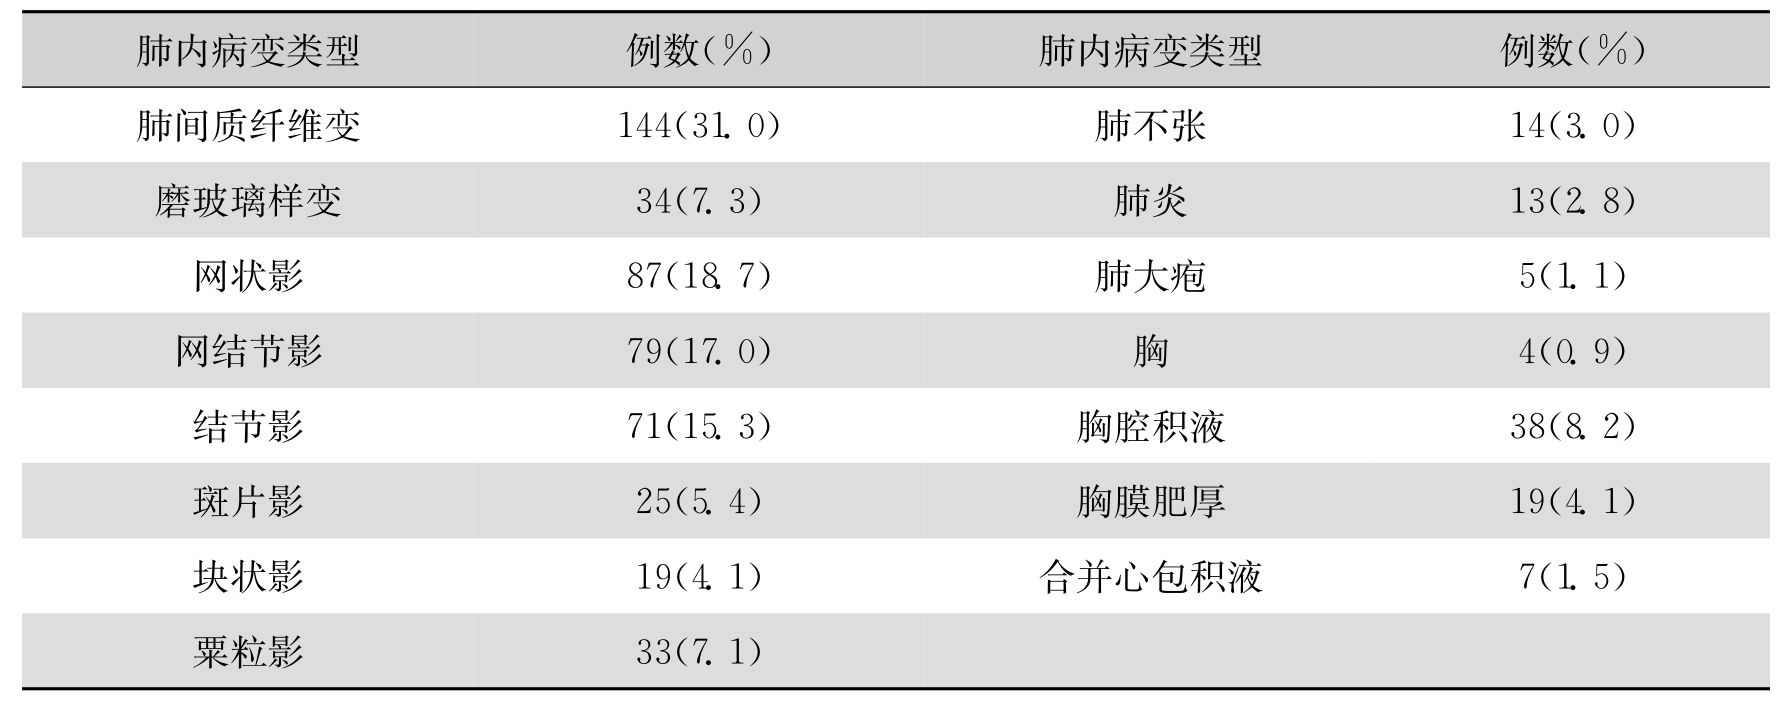
\includegraphics[width=5.92708in,height=2.33333in]{./images/Image00059.jpg}
\end{table}

不典型胸内结节病表现为肺不张、肺内孤立阴影、单侧或双侧肺实变、双肺粟粒样结节、胸腔积液以及单侧纵隔及(或)肺门淋巴结肿大等。须注意与肺门淋巴结结核、淋巴瘤和肺癌以及慢性增殖性结核病、荚膜组织胞浆菌病、波状热或异物性小结节鉴别。结节病的组织学改变是具有类上皮细胞与巨细胞的特别肉芽肿,类似结核病,但无干酪样变,也无结核菌发现,故病理活检有重要诊断价值。慢性增殖性结核病、荚膜组织胞浆菌病、波状热或异物性小结节,都可有类似的病变,须结合其他表现进行鉴别等。下列的临床资料有助于本病诊断:

1.结核菌素试验(PPD),5IU结核菌素的皮肤试验呈阴性或极弱反应,但须注意临床上也存在结节病合并结核病的情况。

2.确定其他器官的结节病病变。对怀疑为本病时,须注意检查其他器官的结节病病变,如多发性囊样骨炎(Jüngling病),X线检查发现指骨有局限性囊状透明区,但无骨膜反应。

3.结节病活动期,血钙增高、血尿酸增加,碱性磷酸酶增高。

4.血管紧张素转换酶(ACE)测定,50\%~75\%的结节病患者血和肺泡灌洗液中ACE水平升高。

5.结节病活动期外周血淋巴细胞减少,而支气管肺泡灌洗液(BALF)中淋巴细胞数明显增多>20\%,CD4/CD8T细胞比值>3.0,对结节病有诊断价值。BALF中的非细胞成分的中性粒细胞趋化因子(NCF)、肿瘤坏死因子(TNF-α)、α2-巨球蛋白(α2-MA)和弹性蛋白酶活性、白介素-2(IL-2)、内皮素-1(ET-1)、纤维连接素(FN)和免疫球蛋白G(IgG)均明显升高,且这些指标均与淋巴细胞百分比呈明显正相关,认为NCF、TNF-α、α\textsubscript{2}
-MA、IL-2、ET-1、FN等均可作为结节病肺泡炎活动性的标志。

6.组织病理学检查
选取肿大浅表淋巴结、纵隔淋巴结、支气管内膜结节进行活检及皮肤损害处活检,典型的病理特征为为非干酪性坏死性上皮细胞样肉芽肿,抗酸染色阴性。这是确诊结节病的主要依据,但必须结合临床考虑。

7.氟代脱氧葡萄糖正电子发射计算机断层显像(\textsuperscript{18} F-FDG
PET)及正电子发射计算机断层显像/计算机断层显像(PET/CT)在结节病诊断、分期及治疗中有一定的应用价值,①能较传统影像学发现更多的结节病累及部位,尤其体格检查、X线胸片或CT等常规方法未发现的隐匿病变部位,如骨骼、后腹膜、颈部及肝脾活动性病变;②评价结节病的活动性,较血清ACE敏感度更高,在血清ACE水平正常时更有价值;③对于指导治疗及评价疗效有价值,肺实质代谢活性增高时需要治疗,并且治疗后能改善肺功能,治疗后病灶的SUV\textsubscript{max}
值降低提示治疗有效,与患者临床症状的改善有相关性;④\textsuperscript{18}
F-FDG和\textsuperscript{11} C-MET
PET联合应用以及双时相\textsuperscript{18} FFDG
PET能提供结节病预后信息;⑤联合应用\textsuperscript{18} F-FDG
PET与\textsuperscript{18} F-FMT PET可鉴别结节病与恶性病变。

\subsubsection{八、血管免疫母细胞性淋巴结病}

免疫母细胞性淋巴结病是一组免疫性淋巴系统疾病,可呈急性、亚急性或慢性经过。本病可有肺部病变,胸片示双侧(或单侧)肺门淋巴结肿大,双肺弥漫性或小结节状阴影,以双下肺为显著,少数病例还有胸腔积液。

\protect\hypertarget{text00081.html}{}{}

\subsection{26.2 单侧肺门增大}

\subsubsection{一、肺门淋巴结结核(参见第26.1节)}

\subsubsection{二、肺部肿瘤}

好发于较大气道或段以上支气管的肺部肿瘤,如原发性支气管癌、支气管类癌、腺样囊性癌(圆柱瘤)和黏液表皮样癌等,常引起单侧肺门或纵隔旁淋巴结肿大,X线检查可发现一侧肺门阴影增大。胸部CT扫描诊断价值更大:①CT能发现普通X线检查不能显示的隐藏部位病灶,特别是心脏后、脊柱旁沟、肺尖、近膈面上下部、侧胸壁处等;②可辨认有无肺门和纵隔淋巴结肿大;③显示肿瘤有无直接侵犯邻近器官;④能发现>3mm的病灶。通过纤维支气管镜检查及病理组织检查有助于确诊,了解不同病理类型。

原发性支气管癌以低分化大小细胞癌及鳞状上皮细胞癌多见。多为一侧肺门类圆形阴影,边缘大多毛糙,有时有分叶表现,或癌肿与转移性肺门或纵隔淋巴结融合而形成单侧性不规则的肺门肿块;也可与肺不张或阻塞性肺炎并存,形成所谓“S”形典型中央型肺癌的X线征象。

支气管类癌、腺样囊性癌(圆柱瘤)和黏液表皮样癌原归属于支气管腺瘤,是来源于气管、支气管上皮及腺体的有恶变倾向的肿瘤,现已废弃支气管腺瘤这一名称。支气管类癌的瘤细胞内含有神经分泌颗粒,可分泌具有激素及生物活性物质,如5羟色胺、组胺和促肾上腺皮质激素等20余种肽类激素,因此部分类癌患者除有呼吸系统症状外,还伴有类癌综合征:皮肤潮红、腹泻、哮喘、心动过速、心瓣膜病和糙皮病,并有毛细血管扩张或出现紫癜等。测定24小时尿5-羟基吲哚乙酸(5-H1AA),尿5-羟基色胺(5-HT)、血小板5-HT及嗜铬粒蛋白A,对诊断或术后的复发判断有意义;腺样囊性癌起源于黏液腺上皮,生长缓慢,多发生于较大的气管;黏液表皮样癌来源于气管、支气管树的唾液腺,较罕见,瘤呈灰色,突出于支气管腔内。它们X线检查早期可无任何特殊改变,如继发局限性肺炎或腺瘤向腔外生长,则可出现单侧肺门增大。胸部CT检查、纤维支气管镜检查及活组织病理检查,有助于诊断。

\subsubsection{三、巨大淋巴结增生症}

本病也称良性淋巴瘤、血管滤泡性淋巴结增生、血管滤泡性纵隔淋巴组织增生、淋巴结错构瘤等,临床上少见,本病可发生在任何年龄,10~45岁多见。发病部位以胸腔多见,易误诊为肺癌、肺炎性假瘤等。突出的临床表现为无痛性淋巴结肿大。病理上分为3型:透明血管型(HV)、浆细胞型(PC)及混合型。外科手术切除是首选治疗方案,由于包块有被膜,划界清楚,易于摘除,术后很少再发。

窦组织细胞增多症(Rosai-Dorfman disease,RDD)
1969年由Rosai和Dorfman首次报道,并将其描述为窦组织细胞增生伴巨大淋巴结病,是一种少见的组织细胞增生性病变。本病多发生于年轻人,典型表现为双侧颈部淋巴结无痛性肿大,可伴有发热、贫血及血沉增快,10\%患者可伴有免疫系统疾病。40\%的患者淋巴结内病变可累及淋巴结外组织器官,如眼眶、头颈部、上呼吸道、皮肤、骨及中枢神经系统。有23\%病例淋巴结外病变为唯一表现,而不伴有其他组织病变。呼吸系统原发性RDD极少见,大多发生于鼻腔鼻窦部,其次为鼻咽部、喉和硬腭。下呼吸道原发性RDD较上呼吸道更为少见。肺原发性RDD文献报道主要为肺门肿物、左肺上叶和下叶肿物。临床表现无特异性,容易与其他肿瘤性或炎症性疾病相混淆。主要表现为胸痛、发热及呼吸困难,影像学显示肺组织内软组织占位性病变;确诊RDD需组织病理学,镜下表现为淋巴细胞、浆细胞浸润,呈窦状排列,组织细胞胞质内可见吞噬的淋巴细胞和中性粒细胞;免疫组织化学染色S-100蛋白及CD68阳性。治疗方式为手术治疗。RDD的预后与病变范围有关,如仅有淋巴结内病变或单一器官病变,疾病有自限性或手术可完全切除者预后较好;如果累及多器官,尤其是重要器官或伴发相关免疫系统疾病,则预后较差。

\protect\hypertarget{text00082.html}{}{}

\section{27 纵隔阴影增宽}

纵隔内任何组织或器官的病变,皆可引起纵隔有块状阴影向外突出,形成纵隔阴影增宽、密度改变和肿物挤压所致的邻近器官移位。纵隔的分区在判断纵隔肿块的来源和性质有重要意义,现以五分法应用较广,上纵隔分前上纵隔、后上纵隔,下纵隔分前、中、后纵隔。X线检查从不同的位置进行观察和摄片肿块所在的部位,对推测肿瘤性质有一定帮助(见图\ref{fig7-1})。

上纵隔肿瘤常见:胸腺瘤、胸内甲状腺肿块、甲状腺旁腺腺瘤;前纵隔肿瘤常见:原发性生殖细胞肿瘤(畸胎瘤)、囊性淋巴管瘤;中纵隔肿瘤常见:纵隔淋巴腺瘤、支气管囊肿、淋巴转移瘤、非霍奇金淋巴瘤、淋巴结结核、心包囊肿;后纵隔肿瘤常见:神经源性肿瘤、食管畸形。

纵隔其他病变包括:纵隔炎、纵隔血肿、纵隔气肿、纵隔脂肪沉积、主动脉瘤。

超声检查能显示前纵隔肿瘤的形象、大小、内部性质,以及其与周围肺、胸膜、心脏、大血管的关系;并能在超声引导下进行活检,以至术前作出定位诊断。

由于纵隔内各种组织层次重叠,普通X线胸片或断层摄片上难以显示病变,CT扫描和磁共振成像(MRI)则可以清晰地显示纵隔内结构变化。CT可通过分析脂肪瘤、囊肿、实体瘤及血管病变间的不同点,对肿块提供较重要的诊断和鉴别诊断资料。

MRI在纵隔肿瘤的诊断中更具有优越性,在人体组织中,以脂肪的MRI信号最强、亮度最大,在图像上呈白色,而纵隔含有大量脂肪,当其他纵隔组织发生肿瘤时,则在白色的强信号背景上形成了鲜明的对照;对于内含液体的各种囊肿性病变,由于其信号强度较固体成分高而易于显示病灶。正电子发射扫描成像已用于纵隔疾病的诊断。

纵隔镜、胸腔镜、纤维支气管镜及超声内镜(EBUS)技术的开展,纵隔淋巴结针刺吸引细胞学检查等为纵隔病变的定性诊断提供重要资料,也可用于某些纵隔病变的手术治疗。

\subsection{27.1 纵隔肿瘤及囊肿}

纵隔肿瘤如体积小,尚无明显压迫邻近器官,则常无症状。但如肿物增大,压迫、侵蚀或贯通邻近组织和器官,则可出现胸痛、咳嗽、胸闷、呼吸困难、吞咽困难、声嘶、上腔静脉阻塞综合征等症状和体征。胸痛多见于神经源性肿瘤;咳嗽多见于畸胎瘤。纵隔良性囊肿大多呈圆形或椭圆形,密度较低,边缘光滑清晰,进展缓慢的阴影。纵隔肿物的定性诊断均有赖于手术切除后行病理学检查。

纵隔淋巴结结核少见,多为成人原发性结核,少数为原发综合征的表现。诊断主要依靠X线胸片及CT或MRI。

各种常见的纵隔肿瘤与囊肿的相互鉴别要点见表\ref{tab7-3}。原发纵隔肿瘤及囊肿的分类及其在国内的发生情况,大致如表\ref{tab7-4}所示。

\subsubsection{一、畸胎瘤及皮样囊肿}

畸胎瘤及皮样囊肿大多位于前纵隔心底部,位于后纵隔者极为少见,呈边缘清楚的、圆形或分叶状肿块阴影。如肿块与周围组织粘连,边缘不整齐,则呈尖刺状突出。恶性者有明显的分叶状。此类肿瘤往往为单侧性,大小不定。如发现肿块内有骨及牙齿阴影,为确诊本病的根据。

畸胎瘤与皮样囊肿可发生于任何年龄,但约3/4病例的症状出现在20~40岁之间。此瘤生长缓慢,常长到相当大时才产生症状。最常见的症状是胸骨后闷胀、胸痛、咳嗽、气短等,这是由于肿瘤压迫、侵蚀、穿透气管、支气管或肺组织引起。如并发感染则多伴咳脓痰与咯血史,易误诊为肺化脓性疾病。如痰中有毛发及皮脂样物质,有助于此瘤的诊断。

\subsubsection{二、神经源性肿瘤}

神经源性肿瘤包括神经纤维瘤、神经节细胞瘤和神经鞘瘤等,是纵隔内最常见的肿瘤之一。可发生于任何年龄,以青年人的发病率最高。临床上约30\%~50\%病例无症状,体格检查时偶然发现,余患者可有胸闷、胸痛、咳嗽等。肋间神经痛、臂丛压迫综合征、霍纳综合征等较少见。

\begin{table}[htbp]
\centering
\caption{几种常见纵隔肿瘤及囊肿的鉴别要点}
\label{tab7-3}
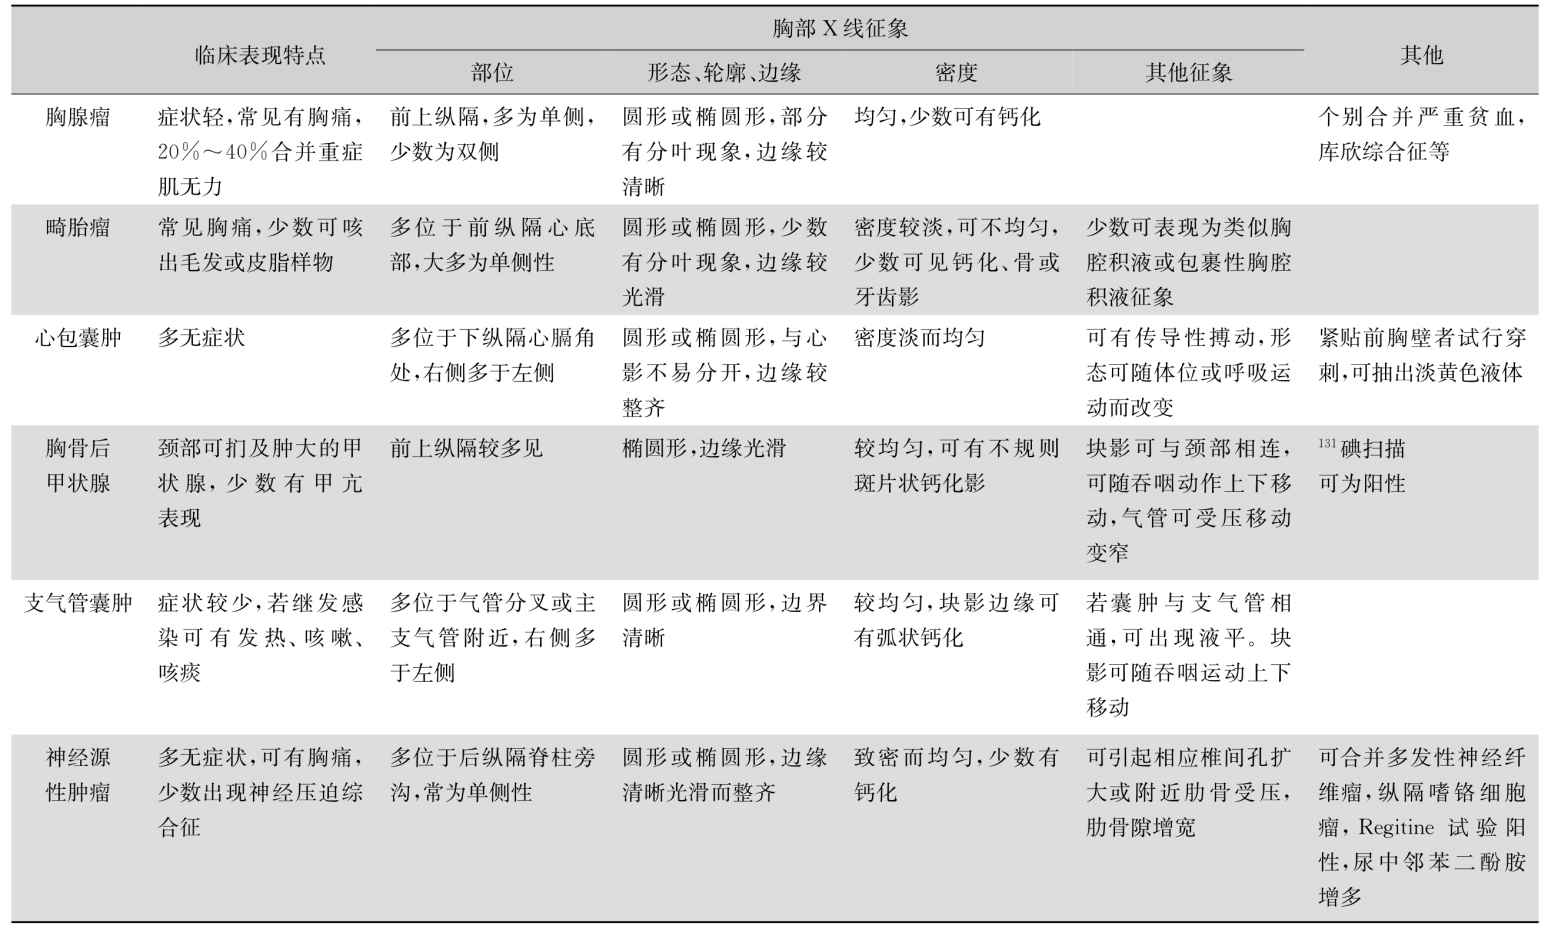
\includegraphics[width=8.76042in,height=5.29167in]{./images/Image00060.jpg}
\end{table}

\begin{table}[htbp]
\centering
\caption{20世纪60~90年代217例纵隔肿瘤各阶段纵隔肿瘤病理分型(例)}
\label{tab7-4}
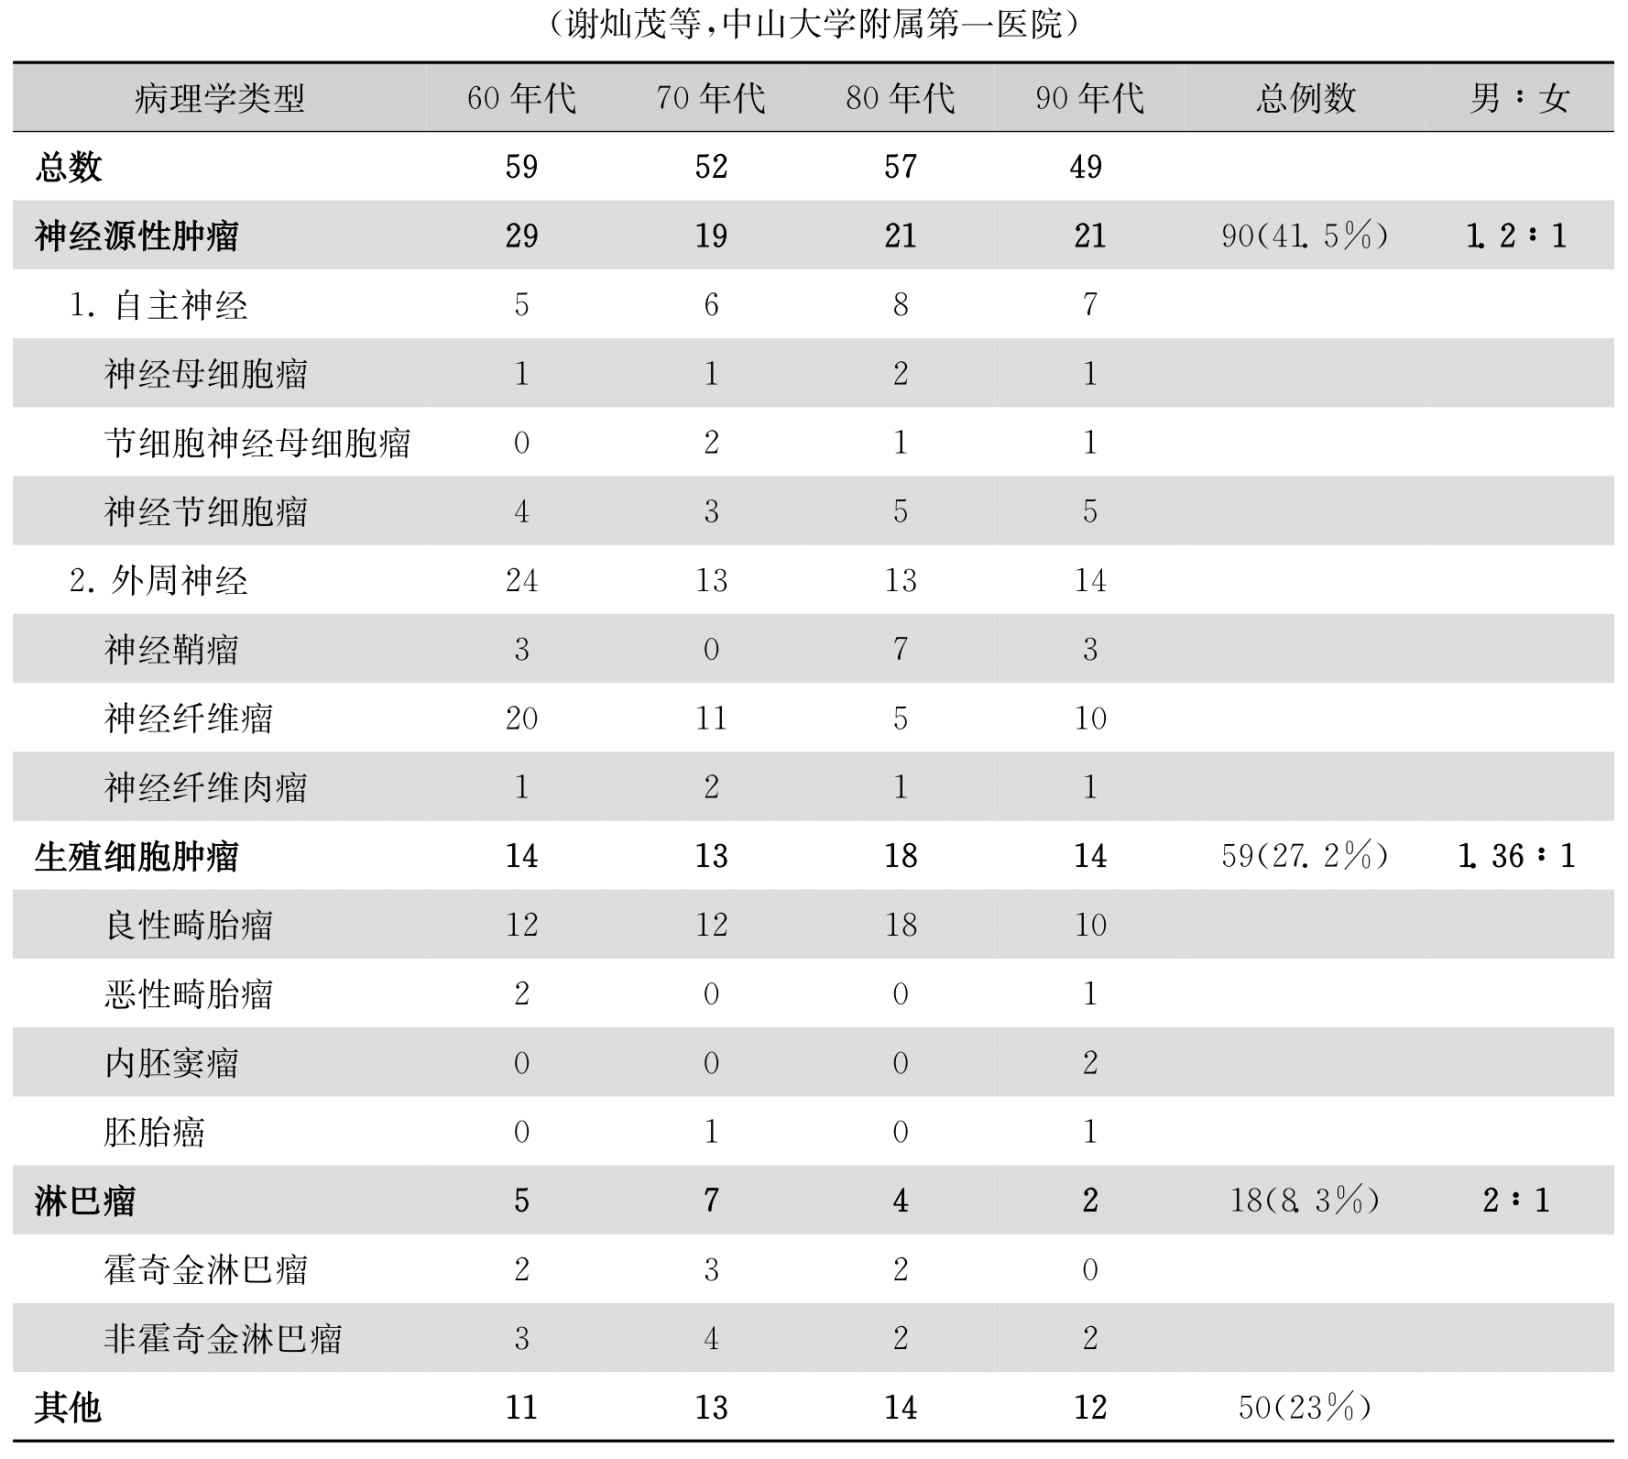
\includegraphics[width=5.91667in,height=5.30208in]{./images/Image00061.jpg}
\end{table}

神经源性肿瘤大多位于后纵隔脊椎旁沟内,少数的神经鞘瘤可位于纵隔中部或前方。X线表现为圆形或卵圆形致密阴影,密度均匀,边界清楚,往往呈单侧性突出,少数有钙化现象。如来自脊髓神经根的肿瘤,同时突入脊髓腔及纵隔,呈哑铃状,常引起椎间孔的增大,位于肋间的可使肋间隙增宽,肋骨缘变形增厚。CT显示于后纵隔脊椎旁有圆形或卵圆形肿块,边缘清楚整齐,少数有钙化和囊性变,有时可见椎骨受压呈现骨质吸收和缺损。MRI呈现在T1加权像上肿瘤信号强度与脊髓相似,在T2加权像上肿瘤信号比脊髓明显增高;肿瘤边界清楚,信号强度均匀一致。在椎骨旁者也可发现椎骨被侵蚀破坏征象。

\subsubsection{三、胸腺肿瘤及囊肿}

胸腺瘤一般位于上前纵隔,在主动脉弓或心底部前方。X线检查时呈圆形或卵圆形边缘整齐的阴影,恶性者有明显分叶状。胸腺肿瘤局部复发及转移的倾向很大,故认为是低度恶性倾向的肿瘤。大部分胸腺瘤为单侧性,密度均匀,少数有钙化区;X线透视下可发现肿块在心脏搏动或呼吸时有移动现象。有报告约30\%~40\%胸腺瘤伴有重症肌无力的表现,注射新斯的明后迅速恢复,有助于此瘤的诊断。CT表现为在血管前间隙有肿块影,圆形或卵圆形,直径1~10cm,一般为软组织密度,可有囊变、钙化,注射照影剂后部分有所增强。MRI表现为在前纵隔有圆形肿块,在T1加权像上肿块信号强度高于肌肉信号强度,在T2加权像上肿块信号强度增高,边界整齐。肿块出现坏死时信号强度不均匀。

胸腺囊肿少见,患者症状轻微或无症状,多于体检行X线透视时发现。X线检查发现上前纵隔囊性肿物时,应考虑此病的可能性。纵隔的囊样肿物,超声检查也有诊断价值。

\subsubsection{四、胸内甲状腺肿块}

胸内甲状腺肿分两类:一类为位于纵隔内而与颈部甲状腺无联系的先天性迷走甲状腺肿,其血供来源于胸腔内动脉,较罕见,约占胸内甲状腺肿块的1\%~3\%;另一类为最常见的继发性胸骨后甲状腺肿,它起源于颈部甲状腺,由于肿大甲状腺的自身重力及胸廓入口以下胸腔负压的吸引,使它沿颈部筋膜向下坠入胸膜腔而形成,它的血供主要来源于甲状腺上或下动脉。胸骨后甲状腺肿位于前上纵隔或后上纵隔,胸部X线可见上纵隔阴影增宽或前上纵隔椭圆形阴影,上缘与颈部相连,气管移向对侧或受压变窄。透视下发现肿块阴影随吞咽动作而上下移动,部分病例的肿块可见钙化影。CT检查可见上纵隔边界清晰与颈部甲状腺相连,CT值高于周围肌肉组织,且密度不均匀,部分有钙化斑或伴气管移位。CT还可明确肿物与气管、食管和大血管的毗邻关系及其与周围组织的粘连情况。如该肿块为有功能的甲状腺组织,放射性核素131碘扫描检查,有助于诊断。约10\%~50\%病例出现甲状腺功能亢进的症状。

\subsubsection{五、纵隔气管支气管囊肿}

纵隔气管支气管囊肿是纵隔先天性发育异常性囊肿中最常见的一种,占40\%~50\%。多发生在后纵隔或中纵隔,依发生部位可分为气管旁、隆突周围、肺门旁、食管旁和其他部位五组。其中大多数位于隆突周围,多有蒂与大气道相连。囊肿多在肺门突出,呈卵圆形或圆形、边缘光滑、密度均匀的致密阴影,部分病例在阴影的边缘可见弧状钙化。X线透视下可见阴影随吞咽而上下移动,或胸膜腔内压改变时囊肿有变形现象。卵圆形密影有时可引起食管局限性压迫移位现象。囊肿较大可产生压迫症状,如气促、缺氧,压迫大气管则出现吸气性呼吸困难及喘鸣。如囊肿与支气管相通,则囊内有气体并出现液平面;如并发感染,则有发热、咳嗽、咳脓痰、胸痛等症状。如囊肿与气管支气管不相通,临床无症状。

\subsubsection{六、淋巴瘤}

淋巴瘤常形成孤立性纵隔肿瘤,并以平滑或波状轮廓为特征。全身症状较明显,从临床表现往往可推测恶性肿瘤的存在。淋巴瘤的下列特点有助于诊断:①症状发展迅速,很快出现上腔静脉与气管受压的症状,部分病例尚有吞咽困难、声带麻痹的表现;②肿瘤首先侵犯中纵隔,后前位X线摄片呈现肺门旁两侧分叶状或结节状肿瘤,边界欠清晰;③对深度X线照射治疗有高度敏感性,往往应用750~1000r的放射治疗量后,肿瘤即迅速缩小乃至消失。

原发性纵隔大B细胞淋巴瘤(PMLBCL)是一种发生于纵隔的、特殊类型的弥漫性大B细胞淋巴瘤,可能为胸腺B细胞来源,具有独特的临床、影像和病理学表现。PMLBCL发生于前上纵隔,肿块的体积巨大(直径>10cm),但无浅表淋巴结及肝脾大等系统性受累表现。临床上一般淋巴瘤的全身症状少见,而以肿瘤局部侵袭产生的压迫症状为主要表现,如气管支气管受压、上腔静脉压迫综合征、胸腔及心包积液等。70\%~80\%的PMLBCL患者血浆LDH升高,是发生中枢神经系统侵犯及预后不良的一个危险因素。

X线表现为上中纵隔影增宽,肿瘤边缘清楚,可呈分叶状。胸部增强CT显示瘤体实性部分轻中度强化,半数患者其内可见液化坏死区。由于PMLBCL病灶体积巨大,心脏和大血管常常被推压、移位非常明显,肿块周围脂肪间隙部分或全部消失,常侵蚀上腔静脉和无名静脉,也可合并胸腔积液、心包积液。需与胸腺瘤、畸胎瘤、内胚窦瘤及纵隔型肺癌等鉴别。

PMLBCL的诊断依靠组织病理学和免疫组织化学,手术和经皮穿刺是常用的活检方法。PMLBCL细胞体积中等至巨大,胞质丰富、透明,细胞核不规则圆形或卵圆形,核仁小,核分裂象较多,有时可见残留胸腺组织,免疫组织化学染色显示肿瘤表达B细胞系特异性表面分子,如CD19、CD20等,而CD3、CD10等阴性,Ki-67阳性率>50\%,提示恶性程度较高。手术治疗不能改善预后,化疗是主要的治疗方法。病变局限于上纵隔,预后相对较好,侵犯胸膜和心包及血浆LDH值明显升高者预后较差。

\subsubsection{七、纵隔原发性绒毛膜癌}

绒毛膜癌(简称绒癌)起源于合体滋养细胞,是一种能分泌HCG的高度恶性肿瘤,可分为:①妊娠性绒癌,又称继发性绒癌,50\%发生在葡萄胎后,30\%发生于流产后,20\%发生于看似正常的妊娠后;为最常见的绒癌类型,化疗效果好;②非妊娠性绒癌,又称原发性绒癌,发生于男性、未婚或绝经后女性的绒癌,极少见,躲在早期发生远处转移,肺为常见转移器官,预后不良。纵隔原发性绒癌主要临床表现为刺激性干咳、胸痛、发热或痰中带血,年龄在20~30岁,X线胸片及胸部CT可见前中上纵隔占位性病变,常伴肺内多发转移灶。临床上不易想到本病,极易误诊,常被误诊为恶性胸腺瘤、畸胎瘤、淋巴瘤、甲状腺癌肺转移。男性患者可见乳房发育,血和尿HCG明显升高,具有较高的特异性及敏感性,其滴度与肿瘤负荷有关,可作为诊断及评估预后的重要指标,通过HCG测定及动态观察,并在B超引导下行纵隔穿刺活检可明确诊断。病理免疫组织化学染色为人绒毛促性腺激素(HCG)阳性,甲胎蛋白(AFP)和CEA阴性,角蛋白上皮细胞阳性。多于早期发生血行转移,且易发生坏死。

\subsubsection{八、纵隔卵黄囊瘤}

卵黄囊瘤又称为内胚窦瘤,是一种由胚外结构------卵黄囊发生的高度恶性生殖细胞肿瘤,发生于性腺器官(卵巢和睾丸),纵隔卵黄囊瘤较少见。多发生于14~35岁男性,临床表现为胸痛、发热、寒战、呼吸困难及上腔静脉阻塞综合征等。体格检查可发现颈静脉怒张、一侧肺呼吸音减低或消失、肝脏肿大、患侧上肢肌力下降等。卵黄囊肿细胞可产生一种特异蛋白------AFP,因此,所有纵隔卵黄囊瘤患者血清AFP水平均明显升高>1000μg/L。X线胸片表现为上中纵隔影增宽,瘤体常较巨大,肿瘤边缘较清,偏向一侧胸腔,部分病例可见胸腔积液。胸部CT表现为前纵隔软组织肿块,密度不均,瘤体内常有出血、坏死及囊变而形成低密度区。增强CT扫描显示肿块不均匀强化,周边强化明显,可出现自周边向中心的不规则条状强化,有的形似血管,这种强化特征在胸腺瘤、淋巴瘤、畸胎瘤等其他纵隔肿瘤中很少见到,对纵隔卵黄囊瘤具有诊断意义。其确诊依靠组织病理学,手术、经皮肺穿刺、彩超引导下活检是常用的活检手段,病理结果较复杂,含有网状、内胚窦样、腺样及实体结构等,免疫组织化学AFP表达阳性。纵隔卵黄囊瘤恶性程度极高,肿瘤生长十分迅速,短期内可发生广泛转移,预后非常差。

\subsection{27.2 急性纵隔炎与纵隔脓肿}

急性纵隔炎是纵隔结缔组织的急性化脓性炎症,多为继发性感染,成年人多见,常出现于食管穿孔、气管破裂、开胸手术、外伤后的感染,口咽部及颈深部的炎症通过器官间隙和筋膜间隙下达纵隔也可引起。纵隔炎病情发展迅速,死亡率高达26.7\%~50\%,因此早期诊断非常重要。临床表现以全身感染中毒症状为主,伴呼吸和吞咽困难,白细胞异常增高。X线表现为纵隔阴影增宽,边缘模糊,纵隔气肿征象,有时可发现脓气胸。侧位观察胸骨后间隙模糊变暗,但无明确的肿块影像。CT表现为纵隔增宽,纵隔内软组织肿胀,纵隔内器官边缘模糊不清,脂肪组织可因炎症渗出而致CT值增高。

纵隔脓肿多由继发感染所致,常见的原因为食管穿孔,少数由纵隔内器官和组织如淋巴结等化脓性感染所引起。颈部和咽部化脓性感染也可沿气管前间隙和椎前间隙向下蔓延至纵隔引起脓肿。发热、胸痛、吞咽困难与呼吸困难是常见症状。白细胞常升高至20
000×10\textsuperscript{9}
/L或以上。脓毒血症症状明显。胸部X线平片呈现纵隔增宽、纵隔内液气面和皮下软组织气带影。CT与MRI检查的诊断价值更大。结核性纵隔脓肿有时不易与肿瘤相鉴别。X线检查如发现颈椎或上段胸椎结核时,可有助于结核性纵隔脓肿的诊断。

\subsection{27.3 主动脉瘤}

主动脉瘤大多为梅毒性与动脉粥样硬化性,最常见于升主动脉,也可发生在主动脉弓部与降主动脉的上端,呈局限性边缘清晰的梭状或囊状致密阴影,在各种不同方向观察下均与主动脉壁紧密不能分开,肿块的边缘与主动脉壁相连贯,与动脉瘤边缘交接处的主动脉壁有被动脉瘤牵引而随之向外膨出的趋向。如主动脉瘤不呈囊状突出,而呈弥漫性仍保持主动脉的外形,则不难与附近肿瘤鉴别。局限性扩张的主动脉瘤与肿瘤鉴别较困难。

局限性梅毒性主动脉瘤常伴有主动脉其他部分的扩张。诊断梅毒性主动脉瘤时,须注意并非所有病例的血清康氏与华氏反应都呈阳性。如同时发现主动脉瓣关闭不全,则支持梅毒性主动脉瘤的诊断。除梅毒外,老年人主动脉粥样硬化所致的主动脉瘤,也可合并主动脉瓣关闭不全。

梅毒性主动脉瘤主要与纵隔肿瘤及中央型支气管肺癌相鉴别。在一般典型病例较易鉴别,个别疑难病例可行CT或MRI、多普勒超声波检查协助诊断。发生在左肺下叶背段的球形支气管肺癌,常易与纵隔衔接而类似升主动脉或降主动脉的主动脉瘤影像,从而引起诊断上的困难。临床上主动脉瘤的胸痛症状较支气管肺癌所致者早,而支气管癌的病程进展较主动脉瘤快;一般中央型支气管肺癌边缘模糊不清,其周围常有肺野的浸润现象,而主动脉瘤则边缘整齐,并与肺野的界限清晰;支气管癌一般不引起食管移位,但可牵拉气管发生移位,而主动脉瘤多引起推挤性移位。鉴别困难时可利用CT以及心血管造影检查。

主动脉造影术与数字减影血管造影术(DSA)是主动脉夹层动脉瘤最可靠的诊断方法,其敏感性近80\%,特异性约95\%。主动脉造影可提供满意的立体像,明确是否有主动脉瓣关闭不全,心脏的充盈与扩张,头臂血管和冠状动脉是否受累的信息。但该检查是有创性检查,且需要经皮动脉插管术以及注射较大量的对比造影剂,因此对于肾功能受损者慎用。

特发性主动脉瘤一般系由先天性动脉中层发育不良引起,常常是马方综合征表现之一,患者多为儿童与青少年,可被误诊为纵隔肿瘤。

\subsection{27.4 心包囊肿与心包憩室}

心包囊肿少见,多为先天性。如囊肿与心包腔连通,称为心包憩室。囊肿呈梭形或卵圆形,直径多为3~8cm,生长缓慢,不致压迫心脏。患者多无自觉症状,囊肿较大时可引起轻度心前区闷痛。

X线平片可见前纵隔心膈角处有一圆形或卵圆形阴影,均质性,边缘光滑,无钙化影,与心脏阴影常不能分开。超声检查可证明肿物为囊性,而非实质性。肿物在X线透视下,吸气时阴影略伸长,而呼气时略扁。立位、侧卧位、头低脚高位可使肿物变形。CT检查有助于明确阴影的囊性结构,但难与主动脉瘤区别时,可考虑行心血管造影术。本病还须与心包包虫囊肿、心室壁瘤鉴别:心包包虫囊肿可根据包虫病的流行病学史、补体结合试验、囊壁钙化现象以及发现体内其他脏器的包虫囊肿等进行鉴别;心室壁瘤一般起源于心肌梗死或外伤,可根据有关的病史、心电图而鉴别之,疑难病例必要时可借助心血管造影术检查。

\subsection{27.5 食管贲门失弛缓症所致的食管扩张}

在食管贲门失弛缓症时,可使贲门上方的食管部分发生高度扩张,从而引起纵隔阴影增宽。患者常有吞咽困难、食物反流等症状。钡餐X线透视易于诊断。

(曾勉 谢灿茂)

\protect\hypertarget{text00083.html}{}{}

\section{参考文献}

1.中华医学会心血管病学分会,中华心血管病杂志编辑委员会.急性心力衰竭诊断和治疗指南.中华心血管病杂志,2010,38:195-208

2.中华医学会心血管病学分会肺血管病学组,中国医师协会心血管内科医师分会.急性肺血栓栓塞症诊断治疗中国专家共识.中华内科杂志,2010,49(1):74-81

3.高元明,等.原发性肺动脉肉瘤的诊断和治疗.中国呼吸与危重监护杂志,2010,09(6):635-638.

4.尚延海,等.白血病胸部浸润的临床X线表现(附68例分析)医学影像学杂志,2002,12(6):449-451

5.董宇杰,等.气管原发性窦组织细胞增多症一例报道并文献复习.中华结核和呼吸杂志,2013,36(7):501-505

6.徐作军.结节病临床诊断方法的评价.中华结核和呼吸杂志,2011,34(7):484-485

7.李多,等.氟代脱氧葡萄糖正电子发射计算机断层显像在结节病诊断及治疗中的应用.中华结核和呼吸杂志,2013;36(6):447-450

8.谢灿茂,等.原发性纵隔肿瘤临床上的几个问题.新医学,1996,8:31-32

9.王星光,等.男性纵隔原发性绒癌肺转移一例.中华结核和呼吸杂志,2013;36(6):464-465

10.牟向东,等.纵隔巨大卵黄囊瘤一例.中华结核和呼吸杂志,2013;36(7):545-546

11.韩海林,等.纵隔炎2例报告.实用放射学杂志,2001,17(2):159-160

12.朱元珏,陈文彬.呼吸病学.北京.人民卫生出版社,2003,1049

\protect\hypertarget{text00084.html}{}{}

